\chapter{Conclusions}
The purpose of the research was to study and analyse different deep learning methods, specifically AutoEncoders and cGANs. The AutoEncoders used were Simple and Global AutoEncoder, both based on the Authors of \cite{deepkoal2017}. Pix2Pix and ChromaGAN were chosen to investigate the performance of cGAN and used to compare against the AutoEncoder methods explored earlier. 

The Places365 dataset was used to train all methods. The dataset consisted of 105,000 samples split into a 60:20:20 ratio. A TensorFlow pipeline was used to help work with the large dataset while having limited memory space. I chose to train the models in Slurm Facility, a service provided by the university that is practically free. 

After a couple of days of training, the methods were tested on the reserved test set and evaluated using objective metrics and Naturalness study. Results have shown that AutoEncoders tend to perform better than cGAN methods using objective metrics, but cGAN performed better on Naturalness Study. 

This raised questions about which evaluation metric matters more. It was noted known that using objective metrics were not reliable when dealing with coloured images as it would only focus on structural and noise difference, not the colour. Hence, the only useful way of evaluating the methods was through human opinion via naturalness study. This study helped conduct a more fair comparison between all methods. The results of the study showed that cGAN was the best deep learning method out of the two compared.




% AutoEncoders are likely biased, as in nearly all cases cGAN manages to perform better in providing more realistic and natural colours. Using historical and colour restoration analysis, and using naturalness study helped reduce this bias and conduct a more fair comparison between all methods. The results of the study showed that cGAN was the best deep learning method out of the two compared.





\section{Future Work}
\subsection{More Data}
One of the limitations seen throughout this project was the time constraint which forced me to limit the dataset to a rather small size of 80,000. And even then, training took a considerable amount of time, taking at most 5 days for training one method (ChromaGAN) for only 20 epochs. Even though \textbf{80,000} may sound a lot in other deep learning tasks, it isn't sufficient enough for the task of Image Colourisation. Having more data will enable the model to achieve a far richer hyperspace to leverage from, which may achieve far more impressive colourisation results.

\subsection{NoGAN training}

\begin{figure}[H]
    \centering
    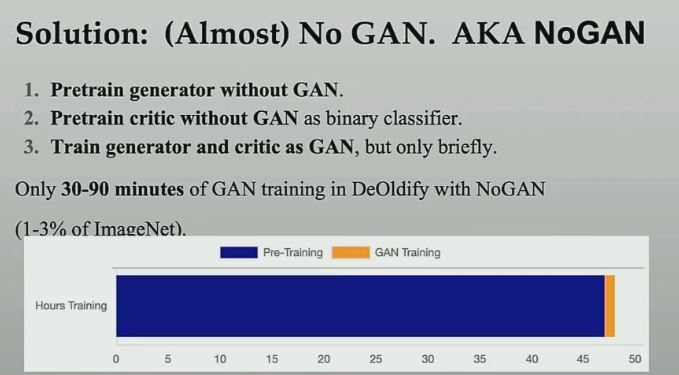
\includegraphics[width=0.8\columnwidth]{sections/figures/nogan.JPG}
    \caption{NoGan training process \cite{nogan2020}}
    \label{fig:my_label}
\end{figure}

NoGAN training is another technique used by the authors of Deoldify \cite{nogan2020}. The process is rather straightforward, you first train the generator model by itself and then generate images from that. You then proceed to use those generated images alongside real images and train the discriminator in a binary classification manner. Finally, you briefly train both the generator and the discriminator together in a GAN setting. The effects of this training method are noted to have reduced the visual abstracts seen prior to this method and have overall improved the colourisation quality. 

\subsection{User guided and Exemplar methods}
\begin{figure}[H]
    \centering
    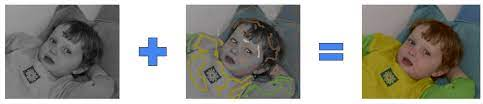
\includegraphics[width=1\columnwidth]{sections/figures/scribble_based_colourisation.jpg}
    \caption{Scribble-based colourisation method which relays on user input \cite{deepimagecolorizationwithuserguidence}}
    \label{fig:my_label}
\end{figure}
Lastly, I would like to experiment with models that involve user guidance. For example, the author's of Scribbler rely on user guidance. The basic process involves scribbling (hence the name) colours onto a chromatic photo. The algorithm will then distribute the colours across regions of the photo. These regions can be anything, such as T-shirts, furniture or landscapes. 

\begin{figure}[H]
    \centering
    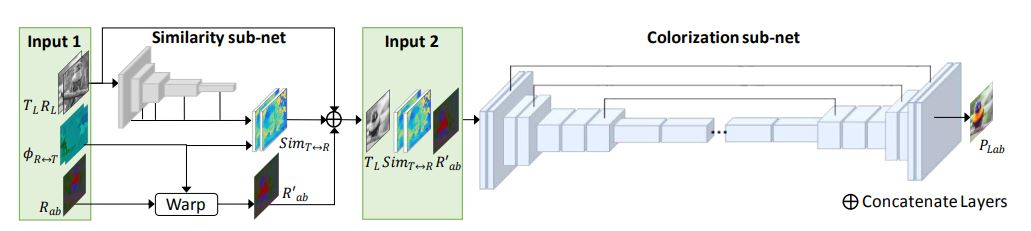
\includegraphics[width=1\columnwidth]{sections/figures/deep_exempler_based_architecture.JPG}
    \caption{Exempler-based architecture for image colourisation \cite{DBLP:journals/corr/abs-1807-06587}}
    \label{fig:my_label}
\end{figure}

In addition to this, I would like to explore ensemble methods that involve combining many models to seek better predictive performance. For example, the author of Deep Exemplar-based Colorization use this technique \cite{DBLP:journals/corr/abs-1807-06587}. 

\section{Self Evaluation}
This research project has allowed me to improve my skills and deepen my interest in the topic of deep learning within the field of Artificial Intelligence. Before beginning this research, I had very little knowledge of AI image colorization or AI in general. The AI and Machine learning modules I took for my third year provided me with the basic foundations I needed to pursue this project. Of course, there were some difficulties along the way: I lacked some key concepts that made understanding certain aspects difficult. However, this was solved after I learnt some of the essential terminologies and concepts. Overall, this project has been an amazing opportunity to learn many new skills and knowledge.

